\section{Chapter 5: Direct and Semidirect Products and Abelian Groups} \label{chap5}

\subsection{Direct Products} \label{sec5.1}

\defi The \textbf{direct product} of groups $G_1, G_2, \ldots, G_n$ with operations $\star_1, \star_2, \ldots, \star_n$ is the Cartesian product $G_1 \times G_2 \times \cdots \times G_n$ with the operation $\star$ defined by
\[(g_1, g_2, \ldots, g_n) \star (h_1, h_2, \ldots, h_n) = (g_1 \star_1 h_1, g_2 \star_2 h_2, \ldots, g_n \star_n h_n).\]
We may extend this to a direct product of infinitely many groups $G_1, G_2, \ldots$ with operation $\star_1, \star_2, \ldots$ whose elements are sequences $(g_1, g_2, \ldots)$.

\prop[Direct Group is a Group] \label{prop5.1}
The direct product of groups $G_1, \ldots, G_n$ is a group with order $|G_1||G_2| \cdots |G_n|$.
\begin{proof}
    To show $G = G_1 \times G_2 \cdots \times G_n$ is a group follows from the fact that each $G_i$ is a group. The identity of $G$ is $(1_1, 1_2, \ldots, 1_n)$ where $1_i \in G_i$ is the identity. The inverse of $(g_1, g_2, \ldots, g_n) \in G$ is $(g_1\inv, g_2\inv, \ldots, g_n\inv)$ where $g_i\inv \in G_i$ is the inverse of $g_i$. The order of $G$ is clear.
\end{proof}

\prop[Projections Onto Direct Groups] \label{prop5.2}
Let $G_1, \ldots, G_n$ be groups with their direct product $G$.
\begin{enumerate}
    \item Fix some $i$. Then
    \[G_i \cong \set{(1, \ldots, 1, g_i, 1, \ldots, 1) \mid g_i \in G_i} \leq G.\]
    Moreover, identifying that subgroup with $G_i$, we have $G_i \nsub G$, and
    \[G/G_i \cong G_1 \times \cdots \times G_{i-1} \times G_{i+1} \times \cdots \times G_n.\]
    \item Define $\pi_i : G \to G_i$ by $\pi_i(g_1, \ldots, g_n) = g_i$. Then $\pi_i$ is a surjective homomorphism with kernel
    \[\ker(\pi_i) = G_1 \times \cdots \times G_{i-1} \times 1 \times G_{i+1} \times \cdots \times G_n.\]
    \item If $g \in G_i$ and $h \in G_j$ for $i \neq j$, then $gh = hg$ in $G$.
\end{enumerate}

\begin{proofnum}
    \item Consider the homomorphism 
    \[\phi : G \to G_1 \times \cdots \times G_{i - 1} \times G_{i + 1} \times \cdots \times G_n, \quad \phi(g_1, \ldots, g_n) = (g_1, \ldots, g_{i - 1}, g_{i + 1}, \ldots, g_n).\] 
    It is easy to see $\ker\phi = \set{(1, \ldots, 1, g_i, 1, \ldots, 1) \mid g_i \in G_i}$ and $\phi$ is surjective. By the First Isomorphism Theorem, (i) is fully proved.
    \item Trivial.
    \item The nonidentity parts of $g$ and $h$ are in different coordinates, so they commute.
\end{proofnum}

\note For $g_i \in G_i$ and $k \in \z$, we have $(g_1g_2\cdots g_n)^k = g_1^kg_2^k \cdots g_n^k$ by \autoref{prop5.2} (iii). Hence,
\[|g_1g_2\cdots g_n| = \lcm(|g_1|, |g_2|, \ldots, |g_n|).\]

\defi The \textbf{elementary abelian} group of order $p^n$ for prime $p$ is the group
\[E_{p^n} = \underbrace{Z_p \times Z_p \times \cdots \times Z_p}_{n \text{ times}}.\]

\subsection{The Fundamental Theorem of Finitely Generated Abelian Groups}

\defi $G$ is \textbf{finitely generated} if some finite $A \subset G$ exists such that $G = \gen A$.

\defi The \textbf{free abelian group of rank $r$} is the direct product of $r$ copies of $\z$, denoted $\z^r$, with $\z^0 = 1$. Moreover, $\z^r = \gen A$, where $A = \set{e_1, e_2, \ldots, e_r}$ and each $e_i$ is the standard basis vector with $1$ in the $i$-th coordinate and $0$ in all other coordinates.
\begin{defn}
    \item We say $G$ is \textbf{finitely generated} if there is a finite subset $A$ of $G$ such that $G = \gen A$.
    \item For every $r \in \z$ with $r \geq 0$, let $\z^r = \z \times \z \times \cdots \times \z$ be the direct product of $r$ copies of $\z$, where $\z^0 = 1$. We call $\z^r$ the \textbf{free abelian group of rank $r$}. The set $A = \set{e_1, e_2, \ldots, e_r}$ where $e_i$ is the element of $\z^r$ with $1$ in the $i$-th coordinate and $0$ in all other coordinates is a generating set for $\z^r$. Moreover, $\z^r$ is abelian since it is a direct product of abelian groups.
    \item In \autoref{theo5.3}, the number $r$ is called the \textbf{Betti number}, or \textbf{free rank} of $G$, and the $n_i$ are called the \textbf{invariant factors} of $G$. The expression $\z^r \times Z_{n_1} \times Z_{n_2} \times \cdots \times Z_{n_s}$ is called a \textbf{factor decomposition} of $G$.
    \item A finite abelian group with invariant factors $n_1, n_2, \ldots, n_s$ such that $n_{i + 1} \mid n_i$ for $1 \leq i \leq s - 1$ has order $n_1 n_2 \cdots n_s$. Moreover, we say that $G$ has \textbf{type} $(n_1, n_2, \ldots, n_s)$.
    \item The integers $p^{\beta_j}$ in \autoref{theo5.5} are called the \textbf{elementary divisors} of $G$. Moreover, the description of $G$ as a direct product of elementary abelian groups is called an \textbf{elementary divisor decomposition} of $G$.
    \item If $G$ is a finite abelian group of type $(n_1, n_2, \ldots, n_s)$, then the \textbf{rank} of $G$ is $s$, or the number of invariant factors of $G$.
    \item If $G$ is any group, then the \textbf{exponent} of $G$ is the minimal positive integer $n$ such that $x^n = 1$ for all $x \in G$. If no such integer exists, then we say that the exponent of $G$ is $\infty$. We denote this number by $\exp(G)$.
\end{defn}

\begin{theo}[Fundamental Theorem of Finitely Generated Abelian Groups]
    \label{theo5.3}
    Let $G$ be a finitely generated group. Then
    \begin{enumerate}
        \item 
        \[G \cong \z^r \times Z_{n_1} \times Z_{n_2} \times \cdots \times Z_{n_s},\]
        for some integers $r, n_1, n_2, \ldots, n_s$ satisfying the following conditions:
        \begin{enumerate}
            \item $r \geq 0$ and $n_j \geq 2$ for all $j$, and
            \item $n_{i + 1} \mid n_i$ for $1 \leq i \leq s - 1$.
        \end{enumerate}
        \item the expression in (1) is unique: if $G \cong \z^t \times Z_{m_1} \times Z_{m_2} \times \cdots \times Z_{m_u}$ for some integers $t, m_1, m_2, \ldots, m_u$ satisfying the same conditions as in (1), then $r = t$, $s = u$, and $n_i = m_i$ for all $i$.
    \end{enumerate}
\end{theo}

\begin{proof}
    The theorem will be derived in \autoref{sec12.1} as a consequence of a more general classification theorem. Finite groups are given an alternate proof at the end of \autoref{sec6.1}.
\end{proof}

\begin{ex}[Listing All Abelian Groups]
    \begin{itemize}
        \item By \autoref{theo5.3}, we may find a way to list all finite abelian groups of a given order. Up to isomorphism, all abelian groups of order $n$ requires that we find all finite sequences of integers $n_1, n_2, \ldots, n_s$ such that
        \begin{enumerate}
            \item $n_j \geq 2$ for all $j \in \set{1, 2, \ldots, s}$,
            \item $n_{i + 1} \mid n_i$ for $1 \leq i \leq s - 1$, and
            \item $n_1 n_2 \cdots n_s = n$.
        \end{enumerate}
        \item Every prime divisor of $n$ must divide the first invariant factor $n_1$.
    \end{itemize}
\end{ex}

\begin{cor}[Distinct Primes Implies Unique Abelian Group]
    \label{cor5.4}
    If $n$ is a product of distinct primes, then up to isomorphism, the only abelian group of order $n$ is the cyclic group of order $n$, $Z_n$.
\end{cor}

\begin{proof}
    Distinct primes imply that no $n_i$ divides the $n_j$ for $j \geq i$, hence the set of number sequences available are only the one sequence $n_1 = n$ and $n_j = 1$ for $j \geq 2$. This corresponds to the cyclic group of order $n$.
\end{proof}

\begin{ex}[Group of Order 180]
    We have $180 = 2^2 \cdot 3^2 \cdot 5$. Note that $2 \cdot 3 \cdot 5 \mid n_1$, so the only choices for $n_1$ are $2^2 \cdot 3^2 \cdot 5$, $2^2 \cdot 3 \cdot 5$, $2 \cdot 3^2 \cdot 5$, and $2 \cdot 3 \cdot 5$. For each choice, we construct potential $n_2$ with $n_2 \mid n_1$ and $n_1n_2 \mid n$. Similarly, we may choose $n_3$ with $n_3 \mid n_2$ and $n_1n_2n_3 \mid n$. We get the following list of sequences:
    \begin{itemize}
        \item $n_1 = 2^2 \cdot 3^2 \cdot 5$, $n_2 = 1$, $n_3 = 1$ corresponds to $Z_{180}$.
        \item $n_1 = 2 \cdot 3^2 \cdot 5$, $n_2 = 2$, $n_3 = 1$ corresponds to $Z_{90} \times Z_2$.
        \item $n_1 = 2^2 \cdot 3 \cdot 5$, $n_2 = 3$, $n_3 = 1$ corresponds to $Z_{60} \times Z_3$.
        \item $n_1 = 2 \cdot 3 \cdot 5$, $n_2 = 6$, $n_3 = 1$ corresponds to $Z_{30} \times Z_6$.
    \end{itemize}
\end{ex}

\begin{theo}[Primary Decomposition Theorem]
    \label{theo5.5}
    Let $G$ be an abelian group of order $n > 1$ and let the unique factorization of $n$ into distinct prime powers be
    \[n = p_1^{\alpha_1}p_2^{\alpha_2} \cdots p_k^{\alpha_k}\]
    Then
    \begin{enumerate}
        \item $G \cong G_1 \times G_2 \times \cdots \times G_k$ where $G_i$ is an abelian group of order $p_i^{\alpha_i}$ for $1 \leq i \leq k$, and
        \item for each $H \in \set{G_1, G_2, \ldots, G_k}$ where $|H| = p^\alpha$, then
        \[H \cong Z_{p^{\beta_1}} \times Z_{p^{\beta_2}} \times \cdots \times Z_{p^{\beta_s}}\]
        where $\beta_1 \geq \beta_2 \geq \cdots \geq \beta_s$ and $\beta_1 + \beta_2 + \cdots + \beta_s = \alpha$.
        \item The decomposition in (1) and (2) is unique: if $G \cong H_1 \times H_2 \times \cdots \times H_k$ where $H_i$ is an abelian group of order $p_i^{\alpha_i}$ for $1 \leq i \leq k$, then $G_i \cong H_i$, and $G_i$ and $H_i$ have the same invariant factors.
    \end{enumerate}
\end{theo}

\begin{proof}
    Proven later.
\end{proof}

\begin{ex}[Classification of Finite Abelian Groups]
    \begin{itemize}
        \item Note that $p^\beta \mid p^\gamma$ if and only if $\beta \leq \gamma$. Moreover, $p^{\beta_1} p^{\beta_2} \cdots p^{\beta_s} = p^\alpha$ if and only if $\beta_1 + \beta_2 + \cdots + \beta_s = \alpha$. The decomposition of $H$ in \autoref{theo5.5}(2) is the invariant factor decomposition of $H$, and the decomposition of $G$ in \autoref{theo5.5}(1) is the primary decomposition of $G$. In particular, the elementary divisors of $G$ are the invariant factors of the Sylow $p$-subgroups of $G$ as $p$ ranges over the prime divisors of $n$.
        \item To find all abelian groups with order $n = p_1^{\alpha_1} p_2^{\alpha_2} \cdots p_k^{\alpha_k}$, we can find all abelian groups of order $p_i^{\alpha_i}$ for $1 \leq i \leq k$ and take their direct products. To find all abelian groups of order $p^\alpha$, we can find all partitions of $\alpha$ and use the partitions to construct the invariant factor decompositions of the groups. In particular, we can obtain all possible lists of invariant factors $p^{\beta_1}, p^{\beta_2}, \ldots, p^{\beta_s}$ by finding all partitions of $\alpha$ into $s$ parts, where $s$ ranges from $1$ to $\alpha$. Moreover, the conditions for invariant factors instead become:
        \begin{enumerate}
            \item $\beta_j \geq 1$ for all $j \in \set{1, 2, \ldots, s}$,
            \item $\beta_{i + 1} \leq \beta_i$ for $1 \leq i \leq s - 1$, and
            \item $\beta_1 + \beta_2 + \cdots + \beta_s = \alpha$.
        \end{enumerate}
        \item The list of invariant factors of an abelian group of order $p^\alpha$ is simply the number of partitions of $\alpha$. In particular, the number of nonisomorphic abelian groups of order $p^\alpha$ is the number of partitions of $\alpha$. For example, abelian groups of order $p^5$ have the following invariant factor decompositions:
        \[
        \begin{array}{c|c}
            \text{Invariant Factors} & \text{Abelian Groups} \\
            \hline
            5 & Z_{p^5} \\
            4, 1 & Z_{p^4} \times Z_p \\
            3, 2 & Z_{p^3} \times Z_{p^2} \\
            3, 1, 1 & Z_{p^3} \times Z_p \times Z_p \\
            2, 2, 1 & Z_{p^2} \times Z_{p^2} \times Z_p \\
            2, 1, 1, 1 & Z_{p^2} \times Z_p \times Z_p \times Z_p \\
            1, 1, 1, 1, 1 & Z_p \times Z_p \times Z_p \times Z_p \times Z_p
        \end{array}\]
        It follows that if $n = p_1^{\alpha_1} p_2^{\alpha_2} \cdots p_k^{\alpha_k}$ such that $a_i$ is the number of partitions of $\alpha_i$ for $1 \leq i \leq k$, then the number of nonisomorphic abelian groups of order $n$ is $a_1 a_2 \cdots a_k$.
    \end{itemize}
\end{ex}

\begin{ex}[Abelian Groups of Order 1800]
    Suppose $n = 1800 = 2^3 \cdot 3^2 \cdot 5^2$. Then we have
    \[
    \begin{array}{c|c|c}
        \text{Order $p^\beta$} & \text{Partitions of $\beta$} & \text{Abelian Groups} \\
        \hline
        2^3 & 3; \quad 2, 1; \quad 1, 1, 1 & Z_{8}, \, Z_4 \times Z_2, \, Z_2 \times Z_2 \times Z_2 \\
        3^2 & 2; \quad 1, 1 & Z_9, \, Z_3 \times Z_3 \\
        5^2 & 2; \quad 1, 1 & Z_{25}, \, Z_5 \times Z_5
    \end{array}\]
    Then we have a total of 12 potential isomorphism types by taking all possible direct products from each abelian group of order $2^3$, $3^2$, and $5^2$:
    \[
    \begin{array}{ll}
        Z_8 \times Z_9 \times Z_{25} & Z_4 \times Z_2 \times Z_3 \times Z_3 \times Z_{25} \\
        Z_8 \times Z_9 \times Z_5 \times Z_5 & Z_4 \times Z_2 \times Z_3 \times Z_3 \times Z_5 \times Z_5 \\
        Z_8 \times Z_3 \times Z_3 \times Z_{25} & Z_2 \times Z_2 \times Z_2 \times Z_9 \times Z_{25} \\
        Z_8 \times Z_3 \times Z_3 \times Z_5 \times Z_5 & Z_2 \times Z_2 \times Z_2 \times Z_9 \times Z_5 \times Z_5 \\
        Z_4 \times Z_2 \times Z_9 \times Z_{25} & Z_2 \times Z_2 \times Z_2 \times Z_3 \times Z_3 \times Z_{25} \\
        Z_4 \times Z_2 \times Z_9 \times Z_5 \times Z_5 & Z_2 \times Z_2 \times Z_2 \times Z_3 \times Z_3 \times Z_5 \times Z_5
    \end{array}\]
\end{ex}

\begin{prop}[Structure of Cyclic Groups]
    \label{prop5.6}
    Let $m, n \in \zp$.
    \begin{enumerate}
        \item $Z_m \times Z_n \cong Z_{mn}$ if and only if $(m, n) = 1$.
        \item If $n = p_1^{\alpha_1} p_2^{\alpha_2} \cdots p_k^{\alpha_k}$ is the unique factorization of $n$ into distinct prime powers, then
        \[Z_n \cong Z_{p_1^{\alpha_1}} \times Z_{p_2^{\alpha_2}} \times \cdots \times Z_{p_k^{\alpha_k}}.\]
    \end{enumerate}
    \begin{proofnum}
        \item Let $Z_m = \gen x$ and $Z_n = \gen y$. Let $\ell = \lcm(m, n)$. Let $x^ay^b \in Z_m \times Z_n$. Then
        \[(x^ay^b)^\ell = x^{a\ell}y^{b\ell} = 1.\]
        Assume by way of contradiction that $(m, n) \neq 1$. Then every element of $Z_m \times Z_n$ has order dividing $\ell < mn$, so $Z_m \times Z_n$ cannot be cyclic, hence not isomorphic to $Z_{mn}$. Conversely, if $(m, n) = 1$, then $\ell = mn$, so $x^ay^b$ has order $\lcm(|x|, |y|) = \lcm(m, n) = mn$. Hence, $Z_m \times Z_n$ is cyclic and isomorphic to $Z_{mn}$.
        \item By induction on $k$. The base case $k = 2$ is given by (1). For the inductive step, we have for some $k \geq 2$ that
        \[Z_{p_1^{\alpha_1}} \times Z_{p_2^{\alpha_2}} \times \cdots \times Z_{p_k^{\alpha_k}} \cong Z_{p_1^{\alpha_1} p_2^{\alpha_2} \cdots p_k^{\alpha_k}}.\] Then
        \[Z_{p_1^{\alpha_1}} \times Z_{p_2^{\alpha_2}} \times \cdots \times Z_{p_k^{\alpha_k}} \times Z_{p_{k + 1}^{\alpha_{k + 1}}} \cong Z_{p_1^{\alpha_1} p_2^{\alpha_2} \cdots p_k^{\alpha_k}} \times Z_{p_{k + 1}^{\alpha_{k + 1}}} \cong Z_n.\qh\]
    \end{proofnum}
\end{prop}

\begin{ex}[Obtaining Elementary Divisors from Invariant Factors]
    If $G$ is an abelian group of type $(n_1, n_2, \ldots, n_s)$, or
    \[G \cong Z_{n_1} \times Z_{n_2} \times \cdots \times Z_{n_s},\]
    Let $n = p_1^{\alpha_1} p_2^{\alpha_2} \cdots p_k^{\alpha_k} = n_1 n_2 \cdots n_s$. We may factor each $n_i$ into its prime factorization
    \[n_i = p_1^{\beta_{i1}} p_2^{\beta_{i2}} \cdots p_k^{\beta_{ik}}\]
    where $\beta_{ij} \geq 0$ for $1 \leq i \leq s$ and $1 \leq j \leq k$. Then by \autoref{prop5.6}(1), we have
    \[Z_{n_i} \cong Z_{p_1^{\beta_{i1}}} \times Z_{p_2^{\beta_{i2}}} \times \cdots \times Z_{p_k^{\beta_{ik}}}.\]
    If $\beta_{ij} = 0$, then $Z_{p_j^0} = Z_1$ is the trivial group, so we can ignore it in the direct product. Hence, the elementary divisors of $G$ are the nontrivial $p_j^{\beta_{ij}}$ for $1 \leq i \leq s$ and $1 \leq j \leq k$. In particular, the elementary divisor decomposition of $G$ is
    \[\prod_{i = 1}^s \prod_{j = 1}^k Z_{p_j^{\beta_{ij}}}.\]
\end{ex}

\begin{ex}[Group of Order 1800]
    If $|G| = 1800 = 2^3 \cdot 3^2 \cdot 5^2$ such that $G$ is type $(30, 30, 2)$, then $G \cong Z_{30} \times Z_{30} \times Z_2$. Since $30 = 2 \cdot 3 \cdot 5$, we have $Z_{30} \cong Z_2 \times Z_3 \times Z_5$. Hence, the elementary divisor decomposition of $G$ is
    \[G \cong Z_2 \times Z_2 \times Z_2 \times Z_3 \times Z_3 \times Z_5 \times Z_5.\]
    where we don't have to maintain the order of $Z_2 \times Z_3 \times Z_5 \cong Z_{30}$ since permutations of the factors in a direct product do not change the isomorphism type of the group.

    Lastly, we may obtain the Sylow $p_j$-subgroups of $G$ by collecting the factors $Z_{p_j^{\beta_{ij}}}$ for $1 \leq i \leq s$. In particular, the Sylow 2-subgroup of $G$ is $Z_2 \times Z_2 \times Z_2$, the Sylow 3-subgroup of $G$ is $Z_3 \times Z_3$, and the Sylow 5-subgroup of $G$ is $Z_5 \times Z_5$.
\end{ex}

\begin{ex}[Obtaining Elementary Divisors From any Cyclic Decomposition]
    If $G$ is a direct product of any number of cyclic groups, then the elementary divisors are just the prime factors of the orders of the cyclic groups. For example, if $G \cong Z_{12} \times Z_{18}$, then the elementary divisors of $G$ are $Z_2$, $Z_2$, $Z_3$, $Z_3$, and $Z_3$ since $12 = 2^2 \cdot 3$ and $18 = 2 \cdot 3^2$. Hence, the elementary divisor decomposition of $G$ is
    \[G \cong Z_2 \times Z_2 \times Z_3 \times Z_3 \times Z_3.\]
\end{ex}

\begin{ex}[Obtaining Invariant Factors From Elementary Divisors]
        Let $G$ be an abelian group of order $n = p_1^{\alpha_1} p_2^{\alpha_2} \cdots p_k^{\alpha_k}$ with a given list of elementary divisors. To find the invariant factors of $G$, we follow the following steps:
    \begin{enumerate}
        \item Group the elementary divisors that are powers of the same prime together. We then obtain $k$ lists of integers, one for each prime $p_j$.
        \item Arrange the integers in nondecreasing order in each list.
        \item Among the $k$ lists, suppose that the longest (the one with the most terms) consists of $t$ integers. If a list has fewer than $t$ integers, then we append $1$'s to the end of the list until it has $t$ integers. We then have $k$ lists of $t$ integers.
        \item For each $i \in \set{1, 2, \ldots, t}$, we multiply the $i$-th integers from each of the $k$ lists together to obtain $n_i$. We then have a list of $t$ integers $n_1, n_2, \ldots, n_t$.
    \end{enumerate}

    Note that the ordering of these lists is structured in such a way to ensure divisibility of the invariant factors. As an example, take $G$ with elementary divisors $2, 3, 2, 25, 3, 2$. We then regroup the elementary divisors into lists of powers of the same prime:
    \[
    \begin{array}{c|c|c}
        p = 2 & p = 3 & p = 5 \\
        \hline
        2 & 3 & 25 \\
        2 & 3 & 1 \\
        2 & 1 & 1
    \end{array}\]
    We then multiply the integers in each row together to obtain the invariant factors $n_1 = 2 \cdot 3 \cdot 25$, $n_2 = 2 \cdot 3 \cdot 1$, and $n_3 = 2 \cdot 1 \cdot 1$. Hence, the invariant factor decomposition of $G$ is
    \[G \cong Z_{150} \times Z_6 \times Z_2\]
    We may refer to the list of the elementary divisors of $G$ after \autoref{defi5.5} to construct a list of the invariant factor decomposition of $G$ using the steps above, where the $i$-th group of the previous list will be isomorphic to the $i$-th group of the following list:
    \[
    \begin{array}{ll}
        Z_{1800} & Z_{300} \times Z_6 \\
        Z_{360} \times Z_5 & Z_{60} \times Z_{30} \\
        Z_{600} \times Z_3 & Z_{450} \times Z_2 \times Z_2 \\
        Z_{120} \times Z_{15} & Z_{90} \times Z_{10} \times Z_2 \\
        Z_{900} \times Z_2 & Z_{150} \times Z_6 \times Z_2 \\
        Z_{180} \times Z_{10} & Z_{30} \times Z_{30} \times Z_2
    \end{array}\]
\end{ex}

\newpage

\subsection{Table of Groups of Small Order}

\begin{defn}
    \item $Z_3 \semidir Z_4$ has order 12 with the presentation
    \[\gen{x, y \mid x^4 = y^3 = 1, x\inv yx = y\inv}\]
    with a normal Sylow subgroup $\gen y$ that is inverted by an element of order 4 acting by conjugation.
    \item $(Z_3 \times Z_3) \semidir Z_2$ has generators and relations
    \[\gen{x, y, z \mid x^2 = y^3 = z^3 = 1, yz = zy, x\inv yx = y\inv, x\inv zx = z\inv}\]
    with a normal Sylow 3-subgroup isomorphic to $Z_3 \times Z_3$, namely $\gen{y, z}$ that is inverted by an element of order 2 acting by conjugation.
    \item $Z_5 \semidir Z_4$ has order 20 with the presentation
    \[\gen{x, y \mid x^4 = y^5 = 1, x\inv yx = y^2}\]
    with a normal Sylow 5-subgroup $\gen y$ that is acted on by an element of order 4 acting by conjugation.
    \item The group $F_{20}$, or the \textbf{Frobenius group of order 20}, has presentation
    \[\gen{x, y \mid x^4 = y^5 = 1, xyx\inv  = y^2}\]
    with a normal Sylow 5-subgroup $\gen y$ that is acted on by an element of order 4 acting by conjugation. Observe:
    \[F_{20} = \gen{(2\ 3\ 4\ 5), (1\ 2\ 3\ 4\ 5).}\]
\end{defn}
The following table lists all abelian groups of order $n$ for $1 \leq n \leq 20$ up to isomorphism: first column is order, second column is the number of nonisomorphic groups of that order, third column is the list of abelian groups of that order, and fourth column is the list of nonabalian groups of that order.
\[
\begin{array}{c|c|c|c}
    n & \text{Number of Groups} & \text{Abelian Groups} & \text{Nonabelian Groups} \\
    \hline
    1 & 1 & Z_1 & - \\
    \hline
    2 & 1 & Z_2 & - \\
    \hline
    3 & 1 & Z_3 & - \\
    \hline
    4 & 2 & Z_4, V_4 & - \\
    \hline
    5 & 1 & Z_5 & - \\
    \hline
    6 & 2 & Z_6 & S_3 \\
    \hline
    7 & 1 & Z_7 & - \\
    \hline
    8 & 3 & Z_8, Z_4 \times Z_2, Z_2 \times Z_2 \times Z_2 & D_8, Q_8 \\
    \hline
    9 & 2 & Z_9, Z_3 \times Z_3 & - \\
    \hline
    10 & 2 & Z_{10} & D_{10} \\
    \hline
    11 & 1 & Z_{11} & - \\
    \hline
    12 & 5 & Z_{12}, Z_6 \times Z_2& A_4, D_{12}, Z_3 \semidir Z_4 \\
    \hline
    13 & 1 & Z_{13} & - \\
    \hline
    14 & 2 & Z_{14}, Z_{7} \times Z_{2} & D_{14} \\
    \hline
    15 & 1 & Z_{15} & - \\
    \hline
    16 & 14 & Z_{16}, Z_8 \times Z_2, Z_4 \times Z_4 & Z_4 \semidir V_4, Z_4 \semidir Z_4, M, D_{16}, QD_{16}, Q_{16} \\
    & & Z_4 \times V_4, Z_2 \times Z_2 \times Z_2 \times Z_2 & D_8 \semidir Z_2, Q_8 \semidir Z_2, D_8 * Z_4 \\
    \hline
    17 & 1 & Z_{17} & - \\
    \hline
    18 & 5 & Z_{18}, Z_6 \times Z_3 & D_{18}, S_3 \times Z_3, (Z_3 \times Z_3) \semidir Z_2 \\
    \hline
    19 & 1 & Z_{19} & - \\
    \hline
    20 & 5 & Z_{20}, Z_{10} \times Z_{2} & D_{20}, Z_5 \semidir Z_4, F_{20}
\end{array}\]

\subsection{Recognizing Direct Products}

\begin{defn}
    \item Let $G$ be a group with $x, y \in G$. Let $A$ and $B$ be nonempty subsets of $G$.
    \begin{itemize}
        \item The \textbf{commutator} of $x$ and $y$ is the element $[x, y] = x\inv y\inv xy$. Note that $[x, y] = 1$ if and only if $xy = yx$.
        \item The \textbf{commutator} of $A$ and $B$ is the set $[A, B] = \gen{[a, b] \mid a \in A, b \in B}$.
        \item The \textbf{commutator subgroup} of $G$ is the subgroup $G' = \gen{[x, y] \mid x, y \in G}$.
    \end{itemize}
    \item Let $H$ and $K$ be normal subgroups of $G$ such that $H \cap K = 1$. Then $HK$ is the \textbf{internal direct product} of $H$ and $K$ in $G$. Conversely, the \textbf{external direct product} of $H$ and $K$ is the group $H \times K$. Note that this distinction is entirely notational because $HK \cong H \times K$ by \autoref{theo5.9}.
\end{defn}

\begin{prop}[Properties of Commutators and the Commutator Subgroup]
    \label{prop5.7}
    Let $G$ be a group with $x, y \in G$, and let $H \leq G$. Then
    \begin{enumerate}
        \item $xy = yx[x, y]$ (in particular, $xy = yx$ if and only if $[x, y] = 1$),
        \item $H \nsub G$ if and only if $[H, G] \leq H$
        \item $\sigma[x, y] = [\sigma(x), \sigma(y)]$ for all $\sigma \in \aut(G)$, $G' \cha G$, and $G/G'$ is abelian.
        \item $G/G'$ is the largest abelian quotient of $G$ in the sense that if $H \nsub G$ and $G/H$ is abelian, then $G' \leq H$. Conversely, if $G' \leq H$, then $H \nsub G$, and $G/H$ is abelian.
        \item If $\phi : G \to A$ is any homomorphism of $G$ into an abelian group $A$, then $\phi$ factors through $G'$, i.e., $G' \leq \ker\phi$ and the following diagram commutes:
        \begin{center}
            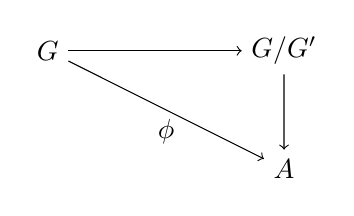
\begin{tikzpicture}[scale = 1.5]
                \node (G) at (0, 0) {$G$};
                \node (GG) at (2, 0) {$G/G'$};
                \node (A) at (2, -1) {$A$};

                \draw[->] (G) to (GG);
                \draw[->] (GG) to (A);
                \draw[->] (G) to node [below] {$\phi$} (A);
            \end{tikzpicture}
        \end{center}
    \end{enumerate}
\end{prop}

\begin{proofnum}
    \item Follows from the definition of the commutator.
    \item Observe that $H \nsub G$ if and only if $g\inv hg \in H$ for all $h \in H$ and $g \in G$. Similarly, for some $h \in H$, then $g\inv hg \in H$ if and only if $h\inv g\inv hg \in H$ so that $H \nsub G$ if and only if $[h, g] \in H$ for every $h \in H$ and $g \in G$. Hence, $H \nsub G$ if and only if $[H, G] \leq H$.
    \item For any $\sigma \in \aut(G)$ with $x, y \in G$, then
    \[\sigma([x, y]) = \sigma(x\inv y\inv xy) = \sigma(x)\inv \sigma(y)\inv \sigma(x)\sigma(y) = [\sigma(x), \sigma(y)].\]
    Hence, $G' = \gen{[x, y] \mid x, y \in G}$ is invariant under $\aut(G)$, so $G' \cha G$. Moreover, for any $x, y \in G$, we have
    \[(xG') (yG') = xyG' = yx[x, y]G' = yxG' = (yG')(xG').\]
    Hence, $G/G'$ is abelian.
    \item If $H \nsub G$ and $G/H$ is abelian, we have that $(xH)(yH) = (yH)(xH)$ for any $x, y \in G$. Then
    \[1H = (xH)\inv (yH)\inv (xH)(yH) = [x, y]H,\]
    so that $[x, y] \in H$ for every $x, y \in G$, and $G' \leq H$.

    If $G' \leq H$, then every subgroup of $G/G'$ is normal because $G/G'$ is abelian by the previous part. In particular, $H/G' \nsub G/G'$, so $H \nsub G$ by the Lattice Isomorphism Theorem. By the Third Isomorphism Theorem, we have
    \[G/H \cong (G/G')/(H/G')\]
    which is abelian since $G/G'$ is abelian.
    \item Similar to (4), we have $G' \leq \ker\phi$ since $\phi([x, y]) = [\phi(x), \phi(y)] = 1$ for all $x, y \in G$. Hence, $\phi$ factors through $G'$, and the diagram commutes.
\end{proofnum}

\begin{ex}[Examples of Commutators and Commutator Subgroups]
    \begin{itemize}
        \item $G$ is abelian if and only if $G' = 1$.
        \item Commutator subgroups can be computed without knowing all calculated commutators. For example, consider $G = D_8$ with $Z(D_8) = \gen{r^2} \nsub D_8$. Then $D_8/Z(D_8)$ is abelian, so $D_8' \leq Z(D_8)$. Since $[r, s] = r\inv s\inv rs = r^2$, we have $D_8' = Z(D_8) = \gen{r^2}$. In particular, a nonabelian group $G$ with order $p^3$ for prime $p$ has commutator subgroup of order $p$, and $G' = Z(G)$.
        \item Let $D_{2n}$ have usual presentation. Since $[r, s] = r^{-2}$, then $\gen{r^{-2}} = \gen{r^2} \leq D'_{2n}$. Moreover, $\gen{r^2} \nsub D_{2n}$ with the images of $r$ and $s$ in $D_{2n}/\gen{r^2}$ generate the quotient. Since they are commuting elements of order $\leq 2$, then the quotient is abelian, and $D'_{2n} \leq \gen{r^2}$. Hence, $D'_{2n} = \gen{r^2}$.
        
        If $n$ is odd, then $\gen{r^2} = \gen r$, whereas even $n$ implies $\gen{r^2}$ has index 2 in $\gen r$. Hence, $D'_{2n}$ is of index 2 or 4 in $D_{2n}$ depending on the parity of $n$.
        \item Since conjugation by $g \in G$ is in $\aut(G)$, then $[a^g, b^g] = [a, b]^g$ for all $a, b \in G$ by \autoref{prop5.7}(3),or conjugates of commutators are also commutators.
        
        As an example in $S_n$, deducing the cycle type of a commutator implies that every element of the same cycle type is also a commutator. In $S_5$, we know that every 5-cycle is a commutator: if we label the vertices of a pentagon as $1, 2, 3, 4, 5$, then $D_{10} \leq S_5$. Then the preceding exercises shows that an element of order 5 is a commmutator in $D_{10}$, so every 5-cycle is a commutator in $S_5$.
    \end{itemize}
\end{ex}

\begin{prop}[Decomposition in Subgroup Products]
    \label{prop5.8}
    Let $H$ and $K$ be subgroups of the group $G$. The number of distinct ways of writing each element of the set $HK$ in the form $hk$ for some $h \in H$ and $k \in K$ is $|H \cap K|$. In particular, if $H \cap K = 1$, then each element of $HK$ can be written uniquely as a product $hk$ for some $h \in H$ and $k \in K$. (This follows from \autoref{prop3.13}).
\end{prop}

\begin{proof}
    Let $x \in HK$. Then $x = h_1k_1$ for some $h_1 \in H$ and $k_1 \in K$. If $x = h_2k_2$ for some $h_2 \in H$ and $k_2 \in K$, then
    \[h_1\inv h_2 = k_1 k_2\inv.\]
    Since the left-hand side is in $H$ and the right-hand side is in $K$, we have that $h_1\inv h_2 \in H \cap K$. Conversely, if $h \in H \cap K$, then
    \[x = h_1 k_1 = (h_1 h) (h\inv k_1) = h_2 k_2\]
    where $h_2 = h_1 h \in H$ and $k_2 = h\inv k_1 \in K$. Hence, there are exactly $|H \cap K|$ distinct ways of writing each element of $HK$ in the form $hk$ for some $h \in H$ and $k \in K$. In particular, if $H \cap K = 1$, then each element of $HK$ can be written uniquely as a product $hk$ for some $h \in H$ and $k \in K$.
\end{proof}

\begin{theo}[Direct Product Recognition Theorem]
    \label{theo5.9}
    Let $G$ be a group with subgroups $H$ and $K$ such that
    \begin{enumerate}
        \item $H \nsub G$ and $K \nsub G$,
        \item $H \cap K = 1$.
    \end{enumerate}
    Then $HK \cong H \times K$.
\end{theo}

\begin{proof}
    By \autoref{cor3.15}, then $HK \leq G$. For $h \in H$ and $k \in K$, observe that normality of $H$ in $G$ implies that $k\inv hk \in H$, so $h\inv k\inv hk \in H$. Similarly, normality of $K$ in $G$ implies that $(h\inv k\inv h)k \in K$. Because $H \cap K = 1$, then $h\inv k\inv hk = 1$, or $hk = kh$ so that $H$ and $K$ commute elementwise. By \autoref{prop5.8}, elements of $H$k are uniquely written as a product $hk$ for $h \in H$ and $k \in K$. Then
    \[\phi : HK \to H \times K \quad \text{defined by} \quad \phi(hk) = (h, k)\]
    is well-defined. Moreover, $\phi$ is a homomorphism since for any $h_1, h_2 \in H$ and $k_1, k_2 \in K$, we have
    \[\phi((h_1k_1)(h_2k_2)) = \phi(h_1 h_2 k_1 k_2) = (h_1 h_2, k_1 k_2) = (h_1, k_1)(h_2, k_2) = \phi(h_1k_1)\phi(h_2k_2).\]
    Finally, $\phi$ is bijective because each $hk$ is uniquely written. Hence, $\phi$ is an isomorphism, and $HK \cong H \times K$.
\end{proof}

\begin{ex}[Examples of Internal Direct Products]
    \begin{enumerate}
        \item Let $n$ be positive and odd. Then $D_{4n} \cong D_{2n} \times Z_2$. Let
        \[D_{4n} = \gen{r, s \mid r^{2n} = s^2 = 1, srs = r\inv}.\]
        Let $H = \gen{s, r^2}$ and $K = \gen{r^n}$. Since $H$ has index 2 (because $H$ contains $s$ and $r^2$ but not $r$), then $H \nsub D_{4n}$. Note that both $s$ and $r$ centralize $r^n$, so $K \leq Z(D_{4n})$, hence $K \nsub D_{4n}$. Note that $K \not\leq H$ since $r^n \notin H$, so $H \cap K = 1$. By \autoref{theo5.9}, then $D_{4n} = HK \cong H \times K$. Since $H$ is generated by an element of order 2 and an element of order $n$ that commute, then $H \cong D_{2n}$, and $K \cong Z_2$. Hence, $D_{4n} \cong D_{2n} \times Z_2$.
        \item Let $I \subseteq \set{1, 2, \ldots, n}$ and $G$ be the setwise stabilizer of $I$ in $S_n$, i.e.,
        \[G = \set{\sigma \in S_n \mid \sigma(i) \in I \text{ for all } i \in I}.\]
        Let $J = \set{1, 2, \ldots, n} \setminus I$. Note that $G$ is also the setwise stabilizer of $J$ in $S_n$. Let $H$ and $K$ be the pointwise stabilizers of $I$ and $J$ in $S_n$, respectively, i.e.,
        \[H = \set{\sigma \in S_n \mid \sigma(i) = i \text{ for all } i \in I}\]
        and
        \[K = \set{\sigma \in S_n \mid \sigma(j) = j \text{ for all } j \in J}.\]
        To see that $H$ and $K$ are normal in $G$, note that if $G$ acts on $I$ and $J$ by permuting the elements, then $H$ and $K$ are the kernels of these actions, so $H$ and $K$ are normal in $G$. Moreover, $H \cap K = 1$ since if $\sigma \in H \cap K$, then $\sigma(i) = i$ for all $i \in I$ and $\sigma(j) = j$ for all $j \in J$, so $\sigma = 1$. By \autoref{theo5.9}, then $G = HK \cong H \times K$. Since $H$ is isomorphic to a subgroup of $S_{n - |I|}$ and $K$ is isomorphic to a subgroup of $S_{|I|}$, then $G \cong S_{n - |I|} \times S_{|I|}$.
        \item Let $\sigma \in S_n$, and let $I$ be the subset of $\set{1, 2, \ldots, n}$ fixed by $\sigma$ pointwise:
        \[I = \set{i \in \set{1, 2, \ldots, n} \mid \sigma(i) = i}.\]
        Let $C = C_{S_n}(\sigma)$. Using Exercise 4.3.18, then $C$ stabilizes $I$ and its complement $J$. Then $C$ is isomorphic to a subgroup $H \times K$, where $H$ is a subgroup of $S_{n - |I|}$ and $K$ is a subgroup of $S_{|I|}$. Noting that $\sigma \in H$, we argue by the preceding example that any $\alpha \in C$ can be written uniquely as $\alpha = \alpha_I\alpha_J$ where $\alpha_I \in H$ and $\alpha_J \in K$. For any $\tau$ that fixes $j \in J$, then $\sigma$ and $\tau$ commute. Then $C$ contains all such $\tau$, or the subgroup $K$. Then $C$ indeed is the set of elements $\alpha_I\alpha_J \in H \times K$ with arbitrary $\alpha_J \in K$ and $\alpha_I$ commutes with $\sigma$:
        \[C = C_H(\sigma) \times K \cong C_{S_J}(\sigma) \times S_I.\]
        In particular, if $\sigma$ is an $m$-cycle, then
        \[C_{S_n}(\sigma) \cong \langle \sigma \rangle \times S_{n-m}.\]
        This has order $m(n - m)!$.
    \end{enumerate}
\end{ex}

\newpage

\subsection{Semidirect Products}

\begin{defn}
    \item Let $H$ and $K$ be groups, and let $\phi : K \to \aut(H)$ be a homomorphism. The \textbf{semidirect product} of $H$ and $K$ with respect to $\phi$ is the group $H \semidir_\phi K$. If the homomorphism $\phi$ is clear from the context, then we simply write $H \semidir K$.
    \item The \textbf{generalized quaternion group of order $2^{n + 1}$} is the group
    \[Q_{2^{n + 1}} = \gen{h, x \mid h^{2^n} = x^4 = 1, x\inv hx = h\inv, h^{2^{n - 1}} = x^2}\]
    for $n \geq 2$.
    \item Let $H$ be a group with $K = \aut(H)$, and $\phi = \id$. Then the semidirect product $H \semidir_\phi K$ is called the \textbf{holomorph} of $H$, denoted $\hol(H)$.
\end{defn}

\begin{theo}[Semidirect Product Construction]
    \label{theo5.10}
    Let $H$ and $K$ be groups, and let $\phi : K \to \aut(H)$ be a homomorphism. Let $\cdot$ be the action of $K$ on $H$ determined by $\phi$. Let $G$ be the set of ordered pairs $(h, k)$ with $h \in H$ and $k \in K$ with the defined multiplication:
    \[(h_1, k_1)(h_2, k_2) = (h_1 (k_1 \cdot h_2), k_1 k_2).\]
    \begin{enumerate}
        \item $G$ is a group with order $|H||K|$.
        \item The sets $\set{(h, 1) \mid h \in H}$ and $\set{(1, k) \mid k \in K}$ are subgroups of $G$ isomorphic to $H$ and $K$ via the maps $h \mapsto (h, 1)$ and $k \mapsto (1, k)$, respectively. We identify these subgroups with $H$ and $K$, or
        \[H \cong \set{(h, 1) \mid h \in H}, \quad K \cong \set{(1, k) \mid k \in K}.\]
    \end{enumerate}
    Upon identification in $G$, we have the following properties:
    \begin{enumerate}[resume]
        \item $H \nsub G$,
        \item $H \cap K = 1$,
        \item for all $h \in H$ and $k \in K$, then $khk\inv = k \cdot h = \phi(k)(h)$.
    \end{enumerate}
\end{theo}

\begin{proofnum}
    \item To see that $G$ is a group, we verify the group axioms:
    \begin{itemize}
        \item Closure: For any $(h_1, k_1), (h_2, k_2) \in G$, then $h_1 (k_1 \cdot h_2) \in H$ and $k_1 k_2 \in K$, so $(h_1 (k_1 \cdot h_2), k_1 k_2) \in G$.
        \item Associativity: For any $(h_1, k_1), (h_2, k_2), (h_3, k_3) \in G$, then
        \begin{align*}
            ((h_1, k_1)(h_2, k_2))(h_3, k_3) &= (h_1 (k_1 \cdot h_2), k_1 k_2)(h_3, k_3) \\
            &= ((h_1 (k_1 \cdot h_2)) ((k_1 k_2) \cdot h_3), (k_1 k_2) k_3) \\
            &= (h_1 ((k_1 \cdot h_2) ((k_1 k_2) \cdot h_3)), k_1 (k_2 k_3)) \\
            &= (h_1 ((k_1 \cdot h_2) (k_1 \cdot (k_2 \cdot h_3))), k_1 (k_2 k_3)) \\
            &= (h_1 (k_1 \cdot (h_2 (k_2 \cdot h_3))), k_1 (k_2 k_3)) \\
            &= (h_1, k_1)((h_2, k_2)(h_3, k_3))
        \end{align*}
        where the fourth equality follows from the definition of a group action.
        \item Identity: $(1, 1)$ is the identity element of $G$ since for any $(h, k) \in G$, then
        \[(1, 1)(h, k) = (1 (1 \cdot h), 1 k) = (h, k)\]
        and
        \[(h, k)(1, 1) = (h (k \cdot 1), k 1) = (h, k).\]
        \item Inverses: For any $(h, k) \in G$, then
        \[(h, k)(k\inv \cdot h\inv, k\inv) = (h (k \cdot (k\inv \cdot h\inv)), k k\inv) = (h h\inv, 1) = (1, 1)\]
        and
        \[(k\inv \cdot h\inv, k\inv)(h, k) = ((k\inv \cdot h\inv) (k\inv \cdot h), k\inv k) = (1, 1).\]
        Hence, $(h, k)\inv = (k\inv \cdot h\inv, k\inv)$.
    \end{itemize}
    \item Let $\wt H = \set{(h, 1) \mid h \in H}$ and $\wt K = \set{(1, k) \mid k \in K}$. Observe that $\wt H$ and $\wt K$ are subgroups of $G$ since for any $h_1, h_2 \in H$ and $k_1, k_2 \in K$, then
    \[(h_1, 1)(h_2, 1) = (h_1 h_2, 1) \in \wt H\]
    and
    \[(1, k_1)(1, k_2) = (1, k_1 k_2) \in \wt K.\]
    Moreover, the maps $h \mapsto (h, 1)$ and $k \mapsto (1, k)$ are isomorphisms since they are bijective homomorphisms. Hence, $\wt H$ and $\wt K$ are subgroups of $G$ isomorphic to $H$ and $K$.
    \item Under the identification of $\wt H$ and $\wt K$ with $H$ and $K$, we see that $K \leq N_G(H)$ since for any $h \in H$ and $k \in K$, then
    \[k\inv hk = (1, k)\inv (h, 1)(1, k) = (k\inv \cdot h, 1) \in H.\]
    Hence, $H \nsub G$.
    \item It is clear that $\wt H \cap \wt K = 1$, so $H \cap K = 1$ under the identification.
    \item For $(1, k) \in \wt K$ and $(h, 1) \in \wt H$, then
    \[(1, k)(h, 1)(1, k)\inv = (1, k)(h, 1)(k\inv \cdot 1, k\inv) = (k \cdot h, 1)\]
    so that $khk\inv = k \cdot h = \phi(k)(h)$ under the identification.
\end{proofnum}

\begin{prop}[Criterion for Equivalence of Semidirect and Direct Products]
    \label{prop5.11}
    Let $H$ and $K$ be groups, and let $\phi : K \to \aut(H)$ be a homomorphism. Then the following are equivalent:
    \begin{enumerate}
        \item The identity (set) map between $H \semidir K$ and $H \times K$ is a group homomorphism, or $H \semidir K \cong H \times K$.
        \item $\phi$ is the trivial homomorphism, i.e., $\phi(k) = 1$ for all $k \in K$,
        \item $K \nsub H \semidir K$.
    \end{enumerate}
\end{prop}

\begin{proof}
    \leavevmode\newline
    $(1) \Rightarrow (2)$: By definition for $h_1, h_2 \in H$ and $k_1, k_2 \in K$ in $H \semidir K$, we have
    \[(h_1, k_1)(h_2, k_2) = (h_1 (k_1 \cdot h_2), k_1 k_2)\]
    If the identity map is a homomorphism, then $(h_1, k_1)(h_2, k_2) = (h_1 h_2, k_1 k_2)$ in $H \times K$. Hence, $h_1 (k_1 \cdot h_2) = h_1 h_2$ for all $h_1, h_2 \in H$ and $k_1 \in K$, so $\phi(k) = 1$ for all $k \in K$.

    \noindent $(2) \Rightarrow (3)$: If $\phi$ is trivial, then the action of $K$ on $H$ is trivial, so the multiplication in $H \semidir K$ is given by
    \[(h_1, k_1)(h_2, k_2) = (h_1 h_2, k_1 k_2)\]
    so that $H \semidir K = H \times K$. Since $K \nsub H \times K$, then $K \nsub H \semidir K$.

    \noindent $(3) \Rightarrow (1)$: If $K \nsub H \semidir K$, then (referencing \autoref{theo5.9}) for all $h \in H$ and $k \in K$, we have $[h, k] \in H \cap K = 1$. Then $kh = hk$, so the action of $K$ on $H$ is trivial, or $\phi(k) = 1$ for all $k \in K$. Hence, the multiplication in $H \semidir K$ is given by
    \[(h_1, k_1)(h_2, k_2) = (h_1 h_2, k_1 k_2)\]
    so that $H \semidir K = H \times K$.
\end{proof}

\begin{ex}[Examples of Semidirect Products]
    Let $H$ and $K$ be groups with homomorphism $\phi : K \to \aut(H)$. Let $G = H \semidir K$, and identify $H$ and $K$ as subgroups of $G$ as in \autoref{theo5.10}(2). We will use \autoref{prop4.16} and \autoref{prop4.17} to determine homomorphisms $\phi$ for specific $H$. The proofs for showing $\phi$ is a homomorphism are omitted, since $K$ will often by cyclic.
    \begin{enumerate}
        \item Let $H$ be abelian (and positively infinite), and let $K = \gen x \cong Z_2$. Define $\phi : K \to \aut(H)$ that maps $x$ to the inverting automorphism of $H$ so that $x \cdot h = h\inv$ for every $h \in H$. Then $G$ contains $H$ as a normal subgroup of index 2, and
        \[xhx\inv = h\inv \quad \text{for all $h \in H$.}\]
        When $H = Z_n$, then $G \cong D_{2n}$, the dihedral group of order $2n$. If $H = \gen z$, then $G = D_\infty$, the infinite dihedral group.
        \item Generalizing the previous example, let $H$ be abelian and $K = \gen x \cong Z_{2n}$. Using the same $\phi$ as before, then $x^2$ acts trivially on $H$. In $G$, we have $xhx\inv = h\inv$, and $x^2hx^{-2} = h$ for all $h \in H$. Then $x^2 \in Z(G)$. If we take $H = Z_3$ and $K = Z_4$, then $G$ is non-abelian of order 12 that is not isomorphic to $A_4$ or $D_{12}$ because its Sylow-2 subgroup, $K$, is cyclic of order 4.
        \item Another generalization of (1) is to let $H = \gen H \cong Z_{2^n}$, $K = \gen x \cong Z_4$ with $xhx\inv = h\inv$. By above, $x^2 \in Z(G)$, and $x$ inverting $H$ implies that $x$ inverts $\gen z$, where $z = h^{2^{n - 1}}$. Then $xzx\inv = z\inv = z$, so $z \in Z(G)$. Then $x^2z \in Z(G)$, or $\gen{x^2z} \nsub G$.
        
        Let $\bar G = G/\gen{x^2z}$. Because $x^2$ and $z$ are distinct commuting elements of order 2, then $|x^2z| = 2$, hence $|\bar G| = 2^{n + 1}$. By factoring out $x^2z$, which implies $x^2 = z\inv = z$, then we may identify $x^2$ and $h^{2^{n - 1}}$ in $\bar G$. For $n = 2$, this implies that $\bar x$ and $\bar h$ are elements of order 4. To see this, suppose $\bar x^2 = 1$. Then $x^2 \in \gen{x^2z}$, so $x^2 = x^2z$ or $x^2 = 1$. Since $z \neq 1$, and $|x| = 4$, this cannot hold. To see that $|\bar h|= 4$, we note that its order divides 4, and $\bar h^2 = \bar x^2 \neq 1$, so its order is 4. We also have that $\bar x$ inverts $\bar h$, and $\bar h^2 = \bar x^2$ is central in $\bar G$. Then $\bar G$ satisfies the same presentation as $Q_8$, so $\bar G \cong Q_8$.

        Suppose $n > 2$. We show that $\bar G$ has a unique subgroup of order 2, namely $\gen{\bar x^2}$. Let $\bar h^i \bar x^j$ be an element in $\bar G$. We split into three cases:
        \begin{itemize}
            \item If $j = 0$, then $\bar h^i$ has order 2 if and only if $\bar h^i = \bar h^{2^{n - 1}} = \bar x^2$.
            \item If $j = 2$, then $(\bar h^i\bar x^2)^2 = \bar h^{2i}$ has order 2 if and only if $\bar h^{2i} = \bar h^{2^{n - 1}} = \bar x^2$, hence $\bar h^i\bar x^2$ has order 4.
            \item If $j = 1$ or $3$, then $\bar x^j$ inverts $\bar h$, so $(\bar h^i \bar x^j)^2 = \bar h^i \bar x^j \bar h^i \bar x^j = \bar h^i (\bar x^j \bar h^i \bar x^{-j}) \bar x^{2j} = \bar h^i \bar h^{-i}\bar x^{2j} = \bar x^2$, so $\bar h^i \bar x^j$ has order 4.
        \end{itemize}

        We claim that $Z(\bar G) = \gen{\bar x^2}$. To see that $\bar x^2 \in Z(\bar G)$, recall that $\bar x^2 = \bar h^{2^{n - 1}}$. This commutes with $\bar h$ trivially, while $\bar x^2$ clearly commutes with $\bar x$. We call $\bar G$ the \textbf{generalized quaternion group} of order $2^{n + 1}$, which is denoted by $Q_{2^{n + 1}}$ with the presentation:
        \[Q_{2^{n + 1}} = \gen{h, x \mid h^{2^n} = x^4 = 1, x\inv hx = h\inv, h^{2^{n - 1}} = x^2}\]
            \item Let $H = (\q, +)$ and $K = \gen x \cong \z$. Let $\phi$ be the map of multiplying by 2 on $H$, hence $x \cdot h = 2h$ for every $h \in H$. Note that $x \z x\inv = 2\z \subset \z$, but $2z \neq \z$, hence $x \not\in N_G(\z)$. This shows that containment is not enough to guarantee normality. 
        \item The semidirect $H \semidir \aut(H)$ is called the \textbf{holomorph} of $H$, denoted $\hol(H)$. Some common holomorphs are:
        \begin{itemize}
            \item $\hol(Z_2 \times Z_2) \cong S_4$,
            \item Let $|G| = n$ and $\pi : G \to S_n$ be the left regular representation. Then $N_{S_n}(\pi(G)) \cong \hol(G)$. Note that the left regular reprsentation of a generator of $Z_n$ is an $n$-cycle in $S_n$, hence
            \[N_{S_n}(\gen{(1\, 2 \ldots n)}) \cong \hol(Z_n) = Z_n \semidir \aut(Z_n)\]
        \end{itemize}
        \item 
    \end{enumerate}
\end{ex}